%!TEX root = ../main.tex


\section{Group-based Acceleration}

As discussed above, we can observe that in Section~\ref{subsec:one}, even with the most efficient imputation-in-the-loop  strategy, \ie  one tuple in  each iteration, the time complexity is  $O(KhnL^2)$, where $K$ is the size of the coreset, $h$ is the sample size, $L$ is a small constant and $n$ is the number of entire dataset. Therefore, obviously, the efficiency is dominated by $n$, which is still low when $n$ is large, and thus it  is necessary to further accelerate this process.

\noindent \textbf{Key observation.}   Recap that in Figure~\ref{fig:overviewSingle}, we can observe that  given a tuple $c$ in the coreset, the tuples in the origin full train set $\trainc$ represented by $c$ are likely to be  closer to each other than other tuples not represented by $c$.
Based on this observation, we propose to first cluster the full train set into groups, and then compute the coreset based on these groups. This can achieve much acceleration because the number of groups is much smaller than $n$. 

At the following, we will theoretically and empirically show the groups-based solution can accelerate the coreset selection process without sacrificing the effectiveness much.

%the acceleration can be achieved by clustering the 

\subsection{Group-based Solution Overview}

\begin{figure}[t]
    \centering
    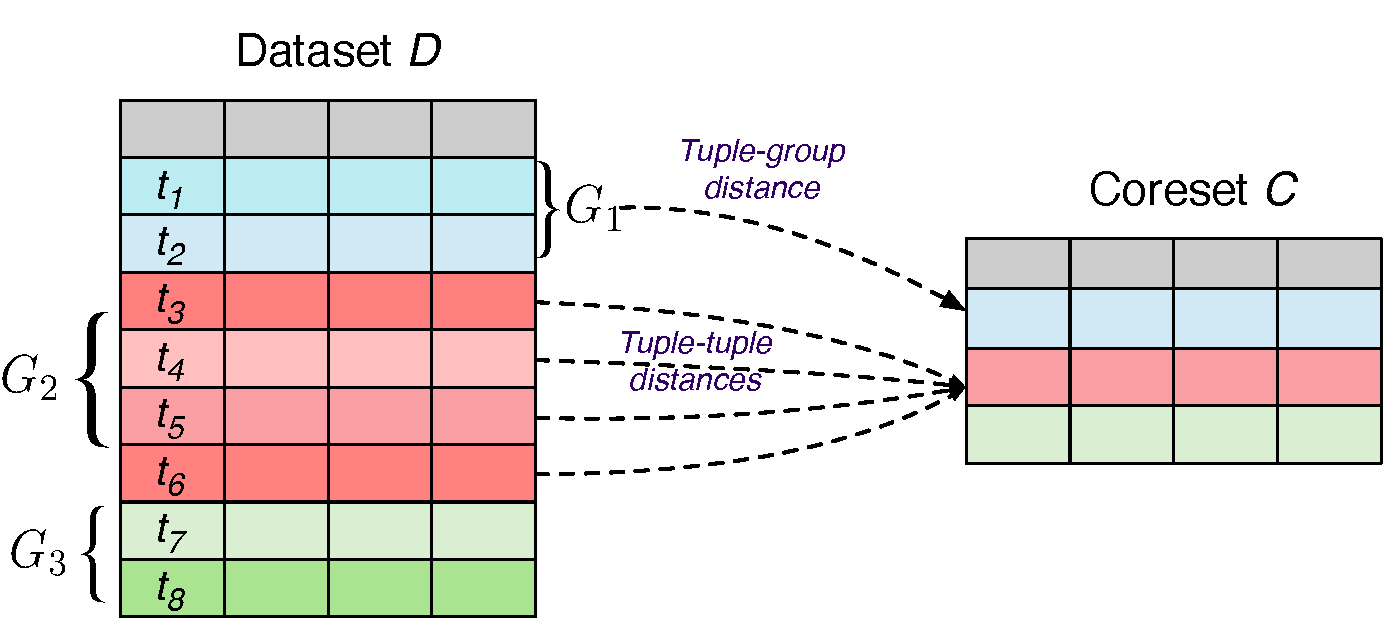
\includegraphics[width=0.6\textwidth]{figs/Overview-gb}
   % \vspace{-2.5em}
    \caption{Illustration of the Group-based Solution.}
    \label{fig:overview-gb}
   % \vspace{-1.5em}
\end{figure}

As shown in Figure~\ref{overview-gb}, one of the core parts of coreset computation is to compute the tuple-tuple distance, \ie $s_{ij}$. For the group-based solution, we just need to consider the relationship between tuples and these pre-computed groups, namely tuple-group distance, rather than the large amount of tuple-tuple distances. As we will discuss below, the computation of tuple-group distance does not need to iterate all tuples in the group, and thus  the overall efficiency can be much improved. 

At a high level, the overall process of group-based \ours solution with imputation in the loop is shown in Algorithm~\ref{alg:group}. To be more explicit, we illustrate Algorithm~\ref{alg:group} in comparison with Algorithm~\ref{alg:framework} in Section~\ref{subsec:framework} without clustering (the modified parts are highlighted in blue fonts).

To be specific, as shown in Line~\ref{alg4:cluster}, we first cluster $\trainc$ into groups using the efficient local sensitive hash (LSH) approach, where each group $\group_u, u\in[1, \groups]$ denotes the indexes of tuples in $\trainc$. In this way, every pair of tuples in the same group is close to each other in the feature distance.
%
 Afterwards, the major difference between group-based \ours and original \ours lies in the 3rd loop. Instead of  selecting a coreset to represent all tuples in the train set, group-based \ours selects a coreset to represent all clusters. As these clusters can well capture the train set distribution, the selected coreset contains enough information to approximate the full gradient of $\trainc$. 
 
 To this end, recap that the typical coreset selection algorithm needs the tuple-tuple distances to approximate the full gradient, while in group-based \ours, we just need to consider the tuple-group distances, \ie  
$\overline{s}_{\gamma(j)u} = \max\limits_{v \in \group_u} s_{\gamma(j)v}, s_{\gamma(j)v} = \lVert\mathbf{x}_v - \mathbf{x}_{\gamma(j)}\rVert, \gamma(j)\in[1, n]$, which denotes the maximum feature distance between the tuple $c_j$ in the coreset and all tuples in $\group_u$. As tuples in $\group_u$ are close to each other, $\overline{s}_{\gamma(j)u}$ can represent the relationship between $c_j$ and tuples in $\group_u$ to a large extent.
%
We will theoretically show that using the maximum distance can still derive a bounded GA error. 
However, since computing $\overline{s}_{\gamma(j)u}$ needs to iterate the tuples in $\group_u$, which is time-consuming, we finally estimate an upper bound $\bound_{jk}$ to compute the coreset score (as shown in Line~11), which still leads to a well-performed coreset. 
%

%!TEX root = ../main.tex

\begin{figure}[!t]
 \vspace{-1em}
	\begin{algorithm}[H]
		\normalem
	\caption{Group-based \ours Solution (imputation-in-the-loop) \label{alg:group}}
		{\small
			
		\KwIn{Incomplete train data $\train$, coreset size $\numcore$, sample size $h$.}
		
		\KwOut{A coreset $\core \subseteq \train$, weight $\weightset=\{w_j\}$,$|\core|=|\weightset|=\numcore$.}
		
		$C=\emptyset$;\\\nllabel{alg1:init1}
		
		\add{Cluster $\train$ into groups $\groups = \{ \group_1, \group_2, ..., \group_\groupsize \}$;}\\\nllabel{alg4:cluster}
		
		\While{$|\core|< \numcore$}
		{\nllabel{craig1:loop1}
			
		/*1st loop*/  \\
		
		Sample $h$ tuples as $T_{sample} \subseteq \train \setminus \core$\\\nllabel{craig1:sample}
		
			\For{each tuple $t \in T_{sample}$}  
			{\nllabel{craig1:loop2}
				
				/*2nd loop*/ \\
				 $\hat{\core} = \core \cup \{t\}$;\\
			%	}
			 %$\mathrm{E}[t|\core]=\texttt{ComputeUtility}(t, C,D)$;
				 %/*3rd loop*/  \\\nllabel{craig1:loop3}
				 \For{\add{each group $G_k \in \groups$}}  
				 {
				 	\add{/*3rd loop*/} \\
				 
				 	%	Get the possible worlds of $\hat{\core} \cup \{t_i\}$;\\\nllabel{one:enumw}
				 	%	Compute $\mathrm{E}[\min_{c_j\in \hat{\core}}s_{ij}]$ using these possible worlds and their probabilities;\\\nllabel{one:exp4pw}
				 		\add{$\mathrm{E}[\hat{\core}] +\!\!= \mathrm{E}[\min_{c_j\in \hat{\core}}\bound_{jk} \times |\group_k|]$, where $\bound_{jk}$ is the upper bound of} \\\quad \\\nllabel{alg4:bound} \add{$\overline{s}_{\gamma(j)k} = \max\limits_{v \in \group_k} s_{\gamma(j)v}, s_{\gamma(j)v} = \lVert\mathbf{x}_v - \mathbf{x}_{\gamma(j)}\rVert, \gamma(j)\in[1, n]$; }\\\nllabel{one:dirtysum}
			     }
		         \add{$\mathrm{E}[t|\core] = \mathrm{E}[\core] - \mathrm{E}[\hat{\core}];$}
				 
			}		

			$t^*$ = $\argmax_{t\in T_{sample}}\mathrm{E}[t|\core]$ ;\\\nllabel{craig1:maxmulti}
			\If{$\mathbb{I}[t^*] = 1$} {\nllabel{craig1:oracle1}
				        Impute $t$ by a  human or automatic method.\\\nllabel{craig1:oracle}
				    }
			$\core = \core \cup \{t^*\}$;
			\\\nllabel{craig1:add2} 
			
				%\If{$\mathbb{I}[t^*] = 1$}
		%	{ \nllabel{alg:if}
		%		 \cc{Impute $t^*$ (by human or automatic methods).}\\\nllabel{alg:oracle}
		%	
			%}					
		}
	 %   \For{ $t\in \core$} 
	  %  {\nllabel{craig1:goodcore1}
	 %      \If{$\mathbb{I}[t] = 1$} {\nllabel{craig1:oracle1}
	 %        Impute $t$ by a  human or automatic method.\\\nllabel{craig1:oracle}
      %       }
     %   }
    
	 	\For{$j = 1$ to $|\core|$} 
	 	{\nllabel{craig1:cc0}
	 		%$w_j = \sum_{i=1}^{n}\mathbb{I}'[j=\argmin_{c_{j'}\in\core}  %\max\limits_{\hypo\in\vartheta}\lVert \df_i(\hypo) - \df_{\gamma(j')}(\hypo) \rVert ]$;\\\nllabel{craig1:cc}
	 		\For{$i = 1$ to n}
	 		{
	 		  \If{$c_j=\argmin_{c_{j'}\in\core}\max\limits_{\hypo\in\vartheta}\lVert \df_i(\hypo) - \df_{\gamma(j')}(\hypo) \rVert$}
	 		  {
	 		  	$w_j~+\!=~1$;\\\nllabel{craig1:cc}
	 		  }
 		    }
	 		
	 	}
		\Return $\core,\weightset$;\\\nllabel{craig1:return}
		}
	\end{algorithm}
\end{figure}




\subsection{Group-based GA Error Bound}

In this section, following the equations in previous sections, we deduce the GA error bound for our group-based solution. 
%
After clustering $\trainc$ to $\{ \group_1 , \group_2, ...\group_U\}$, considering Equation~\ref{eqa:tuple}, we  first rewrite the sum of $n$ feature distances (\ie $\min_{c_j\in \core_k}\lVert\mathbf{x}_i - \mathbf{x}_{\gamma(j)}\rVert$) to $U$ summations. And we use $s_{\gamma(j)v} = \lVert\mathbf{x}_v - \mathbf{x}_{\gamma(j)}\rVert$, as shown in the following Equation:

\begin{equation}\label{eqa:cluster-1}
    \mathrm{E}[C] = \sum_{k= 1}^{|\worlds|} p_k (\sum_{i=1}^n \min_{c_j\in C_k}\lVert\mathbf{x}_i - \mathbf{x}_{\gamma(j)}\rVert) =  \sum_{k= 1}^{|\worlds|} p_k (\sum_{u=1}^U\sum_{v \in \group_u} \min_{c_j\in C_k}\lVert\mathbf{x}_v - \mathbf{x}_{\gamma(j)}\rVert)
\end{equation}

Afterwards, each summation is the sum of $U$ feature distances, as shown in Equation~\ref{eqa:cluster-2},  the sum of each cluster can be bounded by  the maximum distance ($\max_{v \in \group_u} \min_{c_j\in \core_k} s_{\gamma(j)v}$)  multiplying the  cluster size, but the bound is expensive to compute because of iterating $\trainc$. To address this, we further apply the max-min inequality~\cite{} to simplify the computations. 


\begin{equation}\label{eqa:cluster-2}
    \begin{aligned}
        \sum_{k= 1}^{|\worlds|} p_k (\sum_{u=1}^U\sum_{v \in \group_u} & \min_{c_j\in C_k} s_{\gamma(j)v}) \leq \sum_{k= 1}^{|\worlds|} p_k (\sum_{u=1}^U |\group_u| \max_{v \in \group_u} \min_{c_j\in C_k}s_{\gamma(j)v}) \\
        & \leq \sum_{k= 1}^{|\worlds|} p_k (\sum_{u=1}^U |\group_u| \min_{c_j\in C_k} \max_{v \in \group_u}s_{\gamma(j)v}) \\
        & =  \sum_{k= 1}^{|\worlds|} p_k (\sum_{u=1}^U |\group_u| \min_{c_j\in C_k} \overline{s}_{\gamma(j)u})
    \end{aligned}
\end{equation}



Therefore,  we are able to iterate the much smaller cluster $\group$ to compute  the maximum feature distance (\ie $\overline{s}_{\gamma(j)u} = \max_{v \in \group_u}s_{\gamma(j)v}, j \in [1,|\core_k|]$) between each $c_j \in \core_k$ and tuples in each cluster $\group_u$. Then, similar to assigning tuples of the full train set to the tuple of the coreset in previous sections, we can assign the cluster $\group_u$ to the tuple  with the minumum distance, \ie $\min_{c_j\in C_k} \overline{s}_{\gamma(j)u}$. To achieve efficient coreset selection, given $\trainc$ and clusters $\group$, we should precompute all the maximum feature distances $\{\overline{s}_{\gamma(j)u}|j \in [1,N], u \in [1,U]\}$. In this way, we can directly get the value of $\overline{s}_{\gamma(j)u}$.
%
%
%
 %However, as discussed above, computing $\overline{s}_{\gamma(j)u}$ needs to visit every tuple in a cluster, which is still inefficient, so we  efficiently compute an upper bound $\bound_{ju}$ of  $\overline{s}_{\gamma(j)u}$ to replace $\overline{s}_{\gamma(j)u}$. Theoretically, following Eq.~\ref{eqa:cluster-1}, we have:
%
%\begin{equation}\label{eqa:cluster-3}
 %   \begin{aligned}
%        \sum_{k= 1}^{|\worlds|} p_k (\sum_{u=1}^U |\group_u| \min_{c_j\in C_k} \overline{s}_{\gamma(j)u}) \leq \sum_{k= 1}^{|\worlds|} p_k (\sum_{u=1}^U |\group_u| \min_{c_j\in C_k} \bound_{ju})
 %   \end{aligned}
%\end{equation}
%
Similar to Sec~\ref{subsec:exp}, directly computing the probability and getting the expectation is extremely expensive, and thus we still can convert the expectation computation over the possible worlds associated with all clusters to the sum of expectation of each cluster, as follows:

\begin{equation}\label{eqa:cluster-4}
    \begin{aligned}
        \sum_{k= 1}^{|\worlds|} p_k (\sum_{u=1}^U |\group_u| \min_{c_j\in C_k} \overline{s}_{\gamma(j)u}) = \sum_{u=1}^U  |\group_u| \times\mathrm{E}[\min_{c_j\in \hat{\core}}\overline{s}_{\gamma(j)u}]
    \end{aligned}
\end{equation}

\subsection{Algorithm Details}

\vspace{.5em}

\subsubsection{Clustering}~\label{subsec:clustering}
As discussed in Algorithm~\ref{alg:group} Line~2, we need to cluster the entire train set as a pre-processing step. To achieve this efficiently, we adopt the local sensitive hashing~\cite{} to assign similar tuples to the same group. 
%
Note that $\train$ contains some tuples with missing values, an ideal way is to first impute these tuples precisely and then cluster, but we do not know the ground truth in advance. Therefore, we just apply a typical algorithm \ie XXX to impute these missing values, and then conduct the clustering. Although the imputation results may  not be accurate enough, it does not influence much because we just need closer tuples to be included in the same group, and these missing cells do not have a large impact on determining whether two tuples are close. 
%
Finally, tuples with the same hash code are highly similar, which are taken as a cluster,
%
 \add{and it is  efficient to cluster by LSH with a time complexity of  $O(nrm)$, linear with $|\trainc|$.} 
 


\subsubsection{Computing the expected maximum distance.} In this part, we focus on computing Equation~\ref{eqa:cluster-4}, where the key part is the expected maximum distance, \ie $\mathrm{E}[\min_{c_j\in \hat{\core}}\overline{s}_{\gamma(j)u}]$. To be specific, we expand $\mathrm{E}[\min_{c_j\in \hat{\core}}\overline{s}_{\gamma(j)u}] = q_1\min_{c_j\in \hat{\core}}\overline{s}_{\gamma(j)u}^1 + q_2\min_{c_j\in \hat{\core}}\overline{s}_{\gamma(j)u}^2 + ... +q_{card(u)}\min_{c_j\in \hat{\core}}\overline{s}_{\gamma(j)u}^{card(u)}$, where $card(u)$ denotes the number of possible world of $\group_u \cup \hat{C}$, $q_x    (x\in [1, q_{card(u)}])$ denotes the probability of the $x-$th possible world and  $\overline{s}_{\gamma(j)u}^x$ denotes the maximum distance  corresponding to the $x-$th possible world (each possible world does not contain missing values). 
%
%
%
Therefore, to compute the expected maximum distance $\mathrm{E}[\min_{c_j\in \hat{\core}}\overline{s}_{\gamma(j)u}]$, we should know how to compute $\overline{s}_{\gamma(j)u}^x$, \ie the  maximum feature distance between a tuple $c_j$ and a group $\group_u$ within a possible world.

\noindent \textbf{Estimating an upper bound for each possible world.} 
% Given a tuple $c_j\in \hat{C}$ and cluster $\group_u \in \mathcal{G}$, we first brute all possible worlds of $t_v$ and compute the probability(\ie \{$q_1, q_2, ..., q_k$\}) of each possible world(\ie \{$\world_1, \world_2, ..., \world_k$\}). For each possible world $\world_i$, we use $c_j$ denote the tuple and then we can get a tuple-group distance(\ie $s_{jv}$). Then we can use $s_{jv} = \sum_{i=1}^k q_i s_{jv}$ to denote the expectation of tuple-group distance. Formally, following Eq. ~\ref{eqa:cluster-2}, we have:
%
% \begin{equation}\label{eqa:cluster-5}
%     \begin{aligned}
%         |\group_u|  \min_{c_j\in C} \max_{v \in \group_u}s_{\gamma(j)v} = |\group_u|  \min_{c_j\in C} \max_{v \in \group_u} \sum_{i = 1}^{k} q_i s_{\gamma(j)v}
%     \end{aligned}
% \end{equation}
%
For ease of representation, we just use $\overline{s}_{ju}$ to represent  $\overline{s}_{\gamma(j)u}^x$, indicating the maximum feature distance of a possible world.
%
%
 Recap that the reason why we do not directly compute the  $\overline{s}_{\gamma(j)u}$ is that iterating $\group_u$ to compute the maximum distance is expensive.
  To solve this, we propose to leverage the idea of product quantization  to estimate an upper bound $\hat{s}_{ju}$ of $\overline{s}_{ju}$, and then using $\hat{s}_{ju}$ to compute the coreset score still very likely leads to a bounded GA error.
  
  
  
  %We first  introduce the basic concept of PQ widely used in the era of approximate nearest neighbor (ANN) search, which also uses the idea of  decomposing the entire feature space to a Cartesian product of subspaces with low dimensions~\cite{}. Each subspace is quantized separately. Hence, a feature vector can be represented as a short code, and the $a$-th element of the code denotes the  quantization index of the $a$-th subspace of the vector. Finally, in ANN search,  the Euclidean distance between two items can be efficiently estimated from their codes. Next, we will see how to leverage PQ to address our problem.
  
  \noindent  \underline{\textit{Product quantization (PQ)}}  has been widely used for approximate nearest neighbor (ANN) search.  The key idea of PQ is to split the $m$ dimension feature space into a Cartesian product of $M$ low dimensional subspaces, and then quantize each subspace separately.  
 The quantization is conducted by applying $k$-means algorithm~\cite{} over the vectors in each subspace, where $B$ clusters are generated.  
  In this way, a feature vector will be represented as a short code, where the $z$-th element corresponds to the quantization index (\ie cluster ID) of the $z$-th subspace, and thus the Euclidean distance between two vectors can be efficiently estimated based on their short codes. 
  
  
  
  In our scenario, we use the short codes to efficiently estimate an upper bound.
  %
  %
  To be specific, we also split  $\mathbf{x}_{j}$ of $c_j$  into $M$ subvectors, each of which is represented  as $\mathbf{x}^z_{j}$. If we can respectively compute the maximum distance (denoted by $\overline{s}_{ju}^z$) between the $z$-th subvector and vectors in the $z$-th  subspace of $\group_u$, $z\in [1,M]$, and sum them up, we can derive  an upper bound  between $c_j$ and $\group_u$, \ie $ \overline{s}_{ju} \leq  \sum_{z = 1}^M  \overline{s}_{ju}^z$.

%\begin{equation}\label{eqa:cluster-6}
   % \begin{aligned}
    %    |\group_u| \min_{c_j\in C} \max_{v \in \group_u} s_{\gamma(j)v} \leq |\group_u| \min_{c_j\in C} \sum_{a = 1}^M \max_{v \in \group_u} s_{\gamma(j)v}^a
   % \end{aligned}
%\end{equation}

%\noindent we use $s_{\gamma(j)v}^a = \max\limits_{v \in \group_u}\lVert \mathbf{x_v}^a - \mathbf{x}^a_{\gamma(j)}\rVert$ to denote the aforementioned maximum feature distance \wrt the $a$-th subspace. We can take $\bound_{\gamma(j)v}$ as $\sum_{a=1}^{M} s^a_{\gamma(j)v}$. To compute $\bound_{\gamma(j)v}$, next, we  discuss how to efficiently compute  $s_{\gamma(j)}^a, i\in [1,N]$.

 
 

% As shown  in Figure~\ref{}, given the full train data $\trainc$ with $m=$, suppose that we divide it into $M=$ subspaces, each of which has 2 dimensions (the upper part of Figure~\ref{}).  For each subspace, we can sample some tuples and run $k-$means algorithm~\cite{} over this subspace. Suppose that $B$ denotes the number of clusters produced by $k-$means, so in Figure~\ref{}, $\{\bound_1^1, \bound_1^2,..., \bound_1^B\}$ denote the $k-$means cluster centers in the first subspace, associated with indexes (codes) $\{1, 2,...,B\}$. Then, a codebook $c\bound_1$ is computed, which records the feature distance between each pair of cluster centers, and we have $M$ codebooks in total (the lower part of Figure~\ref{}). We use $c\bound_1[x][y]$ to denote the distance between the $x$-th and $y$-th centers. In this way, any $t_i (\mathbf{x}_i) \in \trainc$ can be quantized to a short code $d_i$ with length $M$, and we use $c_i^a, a\in[1,M]$  to denote the $a$-th code, which means the $d_i^a$-th center is the closest one to $\mathbf{x}_i^a$ among all clusters in the $a$-th subspace. For any $t_i, c_j$, their feature distance can be approximated by $s_{ij}=\sum_{l=1}^{M}c\bound_a[d_i^a][d_j^a]$.

% Given $c_j$ and $\group_u$, as shown in Figure ~\ref{}, we compute an approximation of $\hat{s}_{ju}^a$ by first quantizing $\mathbf{x}_{j}$ and $\forall\mathbf{x}_{j} \in \group_u$ to short codes. Then based on the codebooks, for the $a$-th subspace, we compute the largest distance between the corresponding code of $c_j$ and codes of tuples in $\group_u$, \ie $\hat{s}_{ju}^a = \max\limits_{v\in\group_u}cb_a[d_{j}^a][d_u^a]$ as the approximation. Then we approximately compute an upper bound $\bound_{\gamma(j)v}=\sum_{l=1}^{M}\hat{s}_{ju}^a$ by summing the $M$ distances up. Although $\hat{s}_{ju}^a$  may be a little smaller than $s^a_{ju}$ because of the   quantization bias, the above summation $\bound_{ju}$ is always larger than $\overline{s}^a_{ju}$ as each $\hat{s}_{ju}^a$ is close to $s^a_{it}$.

\noindent  \underline{\textit{Computing $\hat{s}_{ju}$ with PQ.}}
Directly computing $\overline{s}_{ju}^z$ still needs to iterate every tuple in $\group_u$, so we leverage these  clusters in each subspace to represent all the vectors in the $z$-th subspace. Since the number of clusters is much smaller than that of all vectors, the efficiency is much improved, which is the key idea of our solution.
%


 Specifically, as shown in Figure~\ref{}, we use $\{\bound_1^1, \bound_1^2,..., \bound_1^B\}$ to represent the  cluster centers in the first subspace. %, associated with indices (codes) $\{1, 2,...,B\}$. 
 Hence, we can build a matrix $mr_1$ to store the feature distances (denoted by $mr_1[x][y]$) between every two cluster center, in total  $M$ matrices are built.  %$c\bound_1[x][y]$ is utilized to denote the distance between the $x$-th and $y$-th centers. 
 %
 %   
 %
 In this way, we can quantize each $t_i (\mathbf{x}_i) \in \mathcal{T}$  to a short code $d_i$, where $d_i^z, z\in[1,M]$  denotes the $z$-th element, indicating that the $d_i^z$-th center has the shortest distance with $\mathbf{x}_i^z$ among all clusters of the $z$-th subspace. 
 Then, the feature distance between  $t_i$ and $c_j$ can then be approximated by $\sum_{z=1}^{M}mr_z[d_i^z][d_j^z]$.

Given $c_j$ and $\group_u$, we approximate $\overline{s}_{ju}^z$ by first quantizing $\mathbf{x}_{j}$ and  $\forall \mathbf{x} \in \group_u$ to short codes. Based on these matrices, for the $z$-th subspace, we compute the maximum distance between the corresponding code of $c_j$ and codes of tuples in $\group_u$, i.e., $\hat{s}_{ju}^z = \max\limits_{v\in\group_u}mr_z[d_{j}^z][d_v^z]$ as the approximation. Then, we approximately compute an upper bound $\hat{s}_{ju}=\sum_{z=1}^{M}\hat{s}_{ju}^z$ by summing the $M$ distances. Although $\hat{s}_{ju}^z$ may slightly underestimate $\overline{s}^z_{ju}$ due to the quantization bias, the summation $\hat{s}_{ju}$ always overestimates $\overline{s}_{ju}$ since each $\hat{s}_{ju}^z$ is close to $\overline{s}^z_{ju}$, leading to a bounded GA error.

\begin{figure}[t]
    \centering
    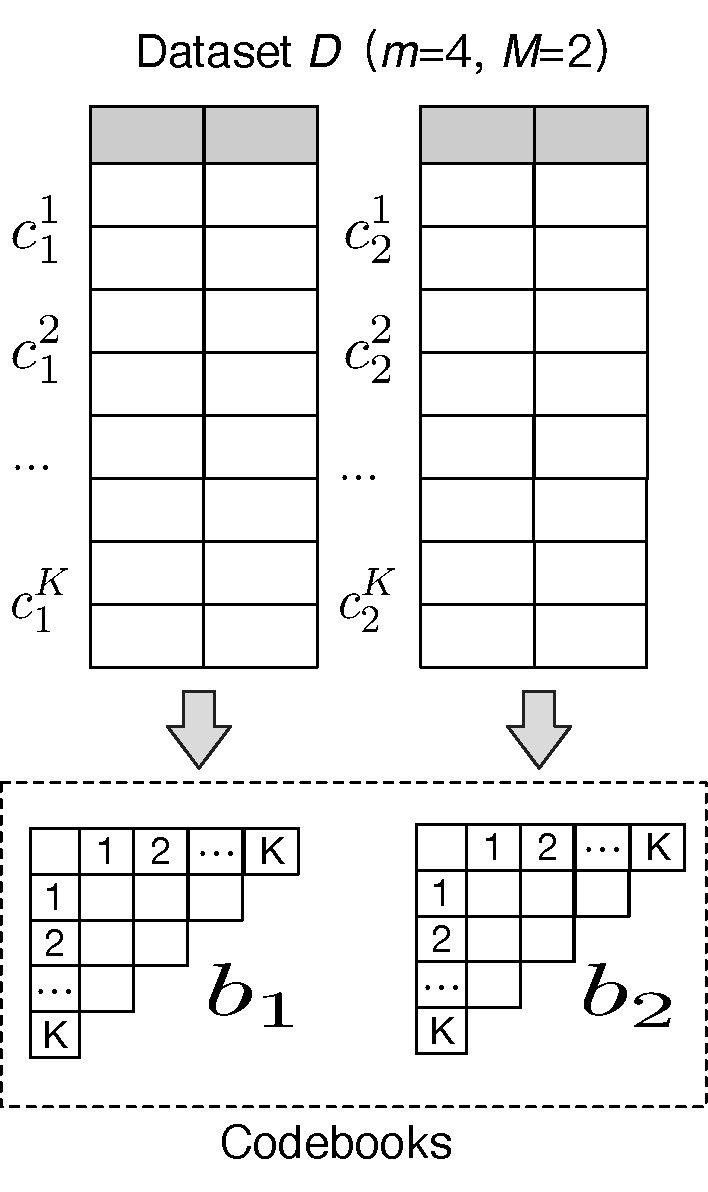
\includegraphics[width=0.3\textwidth]{figs/codebook}
   % \vspace{-2.5em}
    \caption{Illustration of the Group-based Solution.}
    \label{fig:codebook}
   % \vspace{-1.5em}
\end{figure}

\begin{figure}[t]
    \centering
    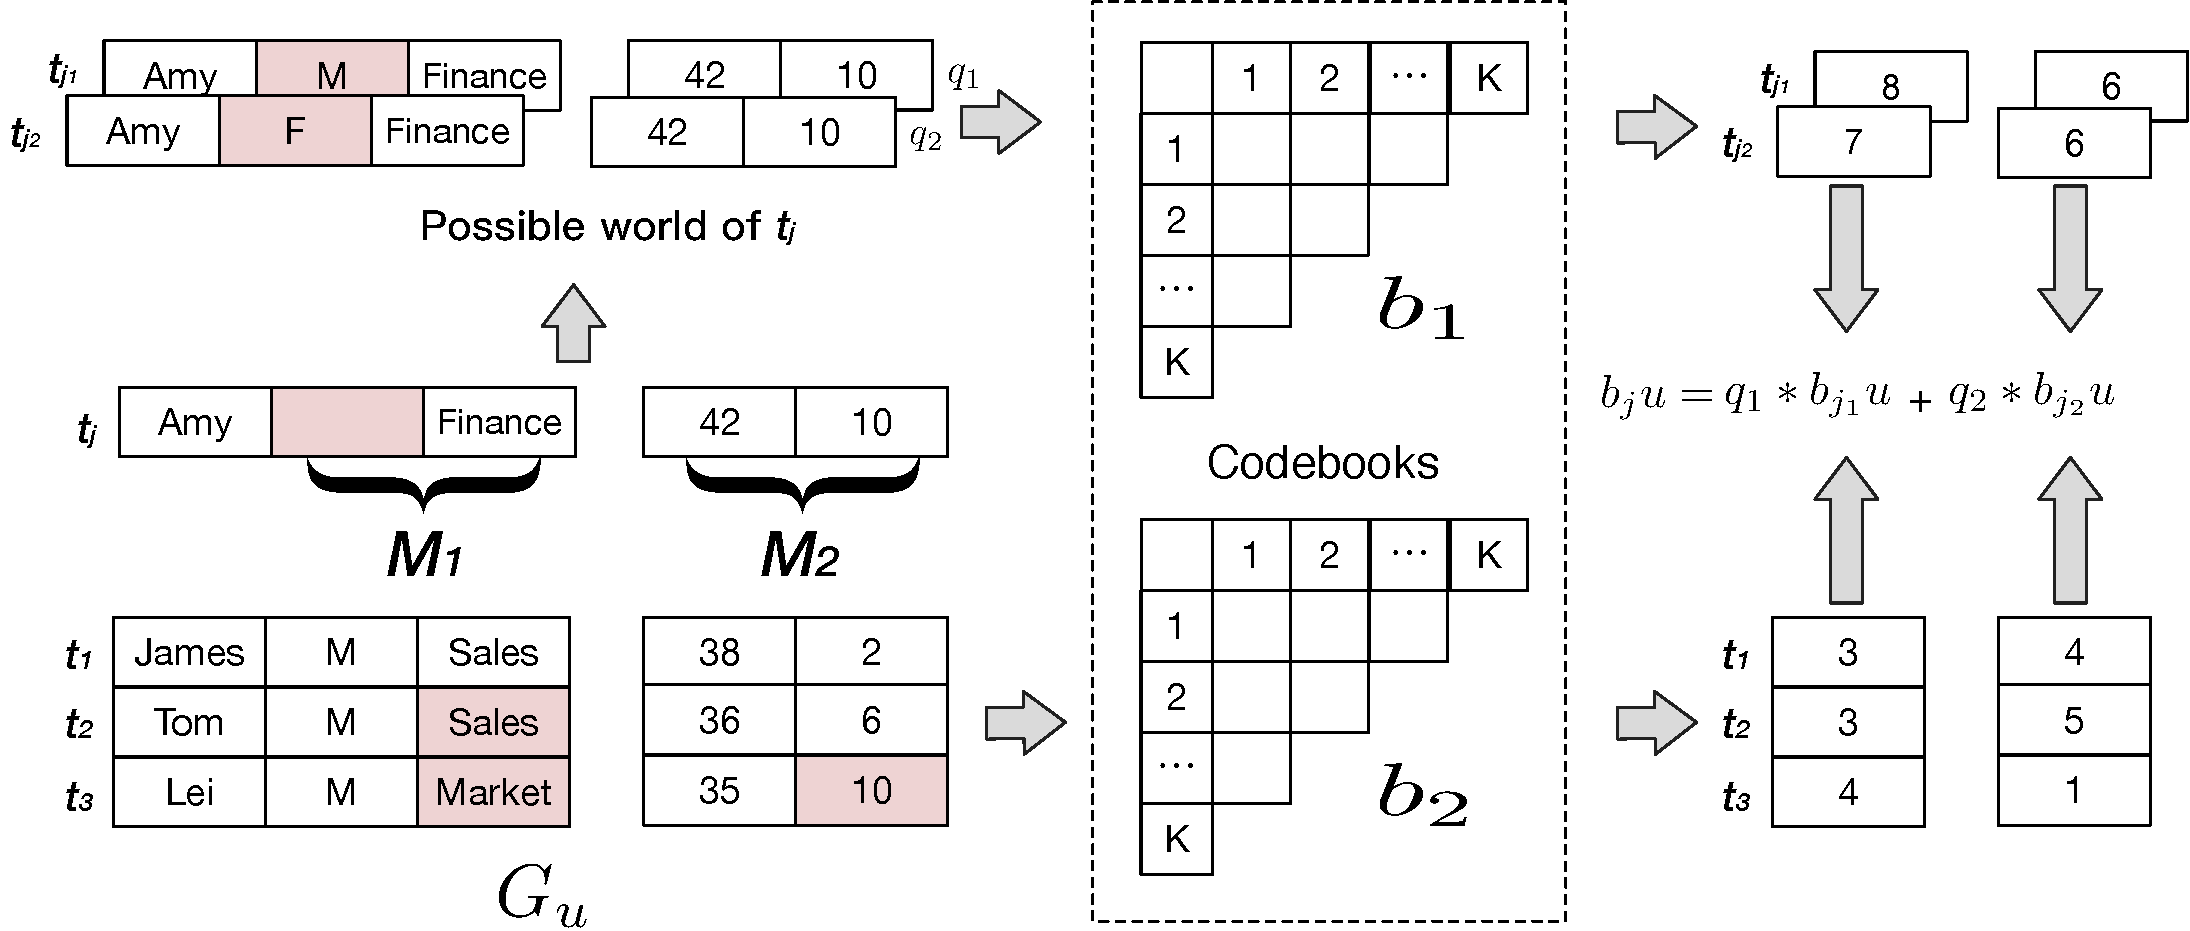
\includegraphics[width=0.8\textwidth]{figs/distance}
   % \vspace{-2.5em}
    \caption{Illustration of the Group-based Solution.}
    \label{fig:distance}
   % \vspace{-1.5em}
\end{figure}

%To cluster $\train$ efficiently,  we use the local sensitive hashing~\cite{} (LSH) to efficiently hash similar tuples to the same group.The basic idea  is to hash $\trainc$ with $r$ random hyperplanes $\{\mathbf{h}_1, \mathbf{h}_2, \dots, \mathbf{h}_r\}$ in the  $m$-dimensional space.Each hyperplane divides the entire space into two half subspaces, and LSH just hashes the  items according to which subspace they fall in. Specifically, for  hyperplane $\mathbf{h}_w, w\in[1,r]$, LSH hashes tuple $t_i\in \trainc$ to hash value 1 if $\mathbf{h}_w \cdot \mathbf{x}_i> 0$, and 0 otherwise. In this way, each $t_i$ is hashed into a $r$-bit 0-1 hash code by $p$ hyperplanes. Since the items with the same hash code are highly similar, we take them as a cluster. Clustering by LSH is highly efficient as it has a complexity of  $O(Nrm)$, linear with $|\trainc|$. 

\noindent \textbf{Time complexity analysis.} First, the cluster centers in PQ can be computed using only a small sampling of $\trainc$, which takes negligible time. Then the codebooks can be computed in $O(mB^2)$ and the short codes of $\trainc$ can be computed in $O(mnB)$. Recap that for the $a$-th subspace the largest distance between corresponding codes of complete $c_j$ and codes of tuples in $\group_u$ without missing values by $\hat{s}_{ju}^a = \max\limits_{v\in\group_u}cb_a[d_{j}^a][d_v^a]$. Since $d_a^j$ only takes from $B$ different values $\{1, 2, \dots, B\}$, we can precompute $\max\limits_{v\in\group_u}cb_a[i][d_v^a], i\in[1, B]$ for each $\group_u$, which takes $O(UB^2)$. In this way, we can compute each $b_{ju}=\sum_{a=1}^{M}\hat{s}^l_{ju}$ in $O(M)$, and all the upper bounds $b_{ju}$, $j\in [1,N]$, $v\in [1,U]$ can be computed in  $O(card(u)MnU)$, much faster than the $O(card(u)mn^2)$. Hence, the overall time complexity is $O()$, which is much faster than $O(KhnL^2)$ because $U \ll n$.

\noindent \textbf{Reducing the number of possible worlds.} Recap that $\mathrm{E}[\min_{c_j\in \hat \core}\bound_{ju}] = \sum_{i=1}^{card(u)} q_i \min_{c_j \in \hat{C}} b_{ju}^i$. However, it is expensive to brute all possible world and compute the probability to get the expectation. To address this issue, one simple way to boost efficiency is by minimizing the number of possible worlds. To achieve this, we can intuitively prioritize possible worlds with higher probabilities, allowing us to discard those with lower probabilities without significantly impacting the accuracy of expectation calculations. It's important to note that the probability of each possible world is determined by multiplying the probabilities of incomplete tuples within that world, as these tuples can be considered independent. Hence, we can eliminate possible worlds containing tuples with low probabilities (\ie reducing $L$), effectively reducing the overall number of possible worlds in the coreset. For example, we can keep top-l(e.g., l = 5) possible worlds (\ie 5 different possible worlds of imputations of $\group$ with high probabilities) of a cluster $\group$. For the number of possible worlds of $\group \cup \hat{C}$, we let $L = L^{\group} * L^t$, where $L^{\group}$ donotes the number of possible worlds of $\group_u$ and $l^t$ denotes the number of possible worlds of $t$.

\noindent \textbf{Generalizing to one batch each iteration.}

